\section{Angular [L]}
\setauthor{Litzlbauer Lorenz}
Um eine nachvollziehbare Auswahl zu treffen, muss verstanden werden, wie Angular funktioniert. 

\subsection{Allgemeines [M]}
\setauthor{Fabian Maar}
Angular ist ein Framework für Webapplikation, das auf der Programmiersprache Typescript basiert. Es ist eines der renommiertesten Frameworks zur Front-End-Entwicklung und wird als Open-Source-Software zur Verfügung gestellt. So besitzt Angular eine große Community und wird von vielen Software-Entwicklern benutzt. So zählt es 2022 zu dem zweitbeliebtesten Front-End Framework \cite{AngularEvidence} und wird von Milliardenkonzernen wie zum Beispiel Google oder PayPal verwendet. 
\cite{AngularEvidence2}

Die große Stärke von Angular ist die Erstellung von Single-Page-Webanwendung, da es eine komponentenbasierte Struktur besitzt. Das bedeutet, der Code ist wiederverwendbar und verkapselt. Komplexe Logiken werden auf ihre Grundelemente reduziert und beeinflussen sich nicht gegenseitig.
\cite{AngularGeneral}

\subsection{Dependencies [L]}
\setauthor{Litzlbauer Lorenz}
In den folgenden Unterabschnitten wird sich mit den Technologien auf die Angular aufgebaut ist, auseinandergesetzt. 
\subsubsection{RxJS}
RxJS ist eine Implementierung von ReactiveX für die Programmiersprache Javascript. Angular verwendet RxJS für reaktive Programmierart.

ReactiveX ist eine Library für das Erstellen von asynchronen und Event-basierenden Programmen, dafür benutzt es  \emph{observable sequences} (Ein beobachtetes Subjekt führt eine Liste von den Observern. Bei einer Veränderung im Subjekt werden die Beobachter nach dieser Liste der Reihe nach informiert. Siehe im Glossar \ref{txt:glos:observerDesignPattern} auf Seite \pageref{txt:glos:observerDesignPattern}).
Die Library arbeitet so mit dem \emph{Observer-Design-Pattern} und fügt verschiedene neue Operatoren hinzu. Zusätzlich werden "Lowlevel"-Funktionen wie Threading, Synchronisation und Thread-Sicherheit verarbeitet und keine Input-/Output-Prozesse blockiert.

\cite{ReactiveXIntro}
\subsubsection{Webpack}
\setauthor{Litzlbauer Lorenz}
Die Hauptfunktion von Webpack ist es, viele verschiedene Daten zu einem Paket für eine JavaScript Applikation zusammenzufassen.
Angular benutzt Webpack, um TypeScript in JavaScript und Sass bzw. Scss in Css umzuwandeln. Beim Bauen des Projektes werden alle Module in ein einziges zusammengefasst. Bei der Entwicklung der Applikation wird durch Webpack \emph{Live-Reloading} unterstützt. Dabei wird bei einer Änderung im Code die gesamte Applikation aktualisiert und neu gestartet.

\subsection{Vorteile/Auswahlkriterien [M]}
\setauthor{Fabian Maar}
Folgende Aspekte sprechen für die Nutzung Angular in diesem Projekt:

\begin{itemize}
  \item komponentenbasiertes Programmieren;
  im Abschnitt \ref{components} wird nochmals deutlich, wie dieser Aspekt genutzt wird.
  \item einfache und übersichtliche Einbindung von Libraries durch ngModules; wird behandelt in Kapitel NgModules \ref{sec:NgModules} 
  \item Isolierung der Logik mit der Benutzeroberfläche durch die Model-View-Controller Architektur und die Model-View-Viewmodel Architektur; wird behandelt in Kapitel MVC und MVVM \ref{sec:MVCandMVVM} 
  \item 
  Dependency Injection für die Verbindung von Front-End zum Back-End; siehe Kapitel HTTP Services \ref{DPI}
\end{itemize}

\subsection{Model-View-Controller und Model-View-ViewModel Architecture [M]}\label{sec:MVCandMVVM}
\setauthor{Fabian Maar}
\subsubsection{Allgemein}

Angular basiert auf dem Konzept des Model-View-Controller- (MVC) und Model-View-ViewModel (MVVM) Architecture Patterns. Diese Patterns werden verwendet, um die Logik von der Benutzeroberfläche zu trennen und komplexe Aufgaben einfacher zu bewältigen. Dies wird in der Fachsprache auch oft als "Separation of Concerns” bezeichnet.
\cite{AngularArchitecturePattern}

Architecture Patterns sind Muster, die verwendet werden um:
\begin{itemize}
  \item eine Software-Anwendung zu strukturieren
  \item die Redundanz von wiederholenden Code-Teile zu vermeiden 
  \item immer wiederkehrende Probleme durch eine einmalige Lösungen zu beheben
  \item um die Wartung und Testung zu erleichtern
  \item Änderungen am Umfang und der Größe der Applikation leichter handhaben zu können
\end{itemize}

\cite{MVCmdn}
\cite{MVVM}
\cite{MVC}

\subsubsection{Model-View-Controler (MVC)}
Die ”Separation of Concerns” wird bei diesem Pattern durch die Aufteilung der Applikation in Model, View und Controller realisiert. Dadurch ist es möglich, sich auf einen Aspekt der Implementierung zu fokussieren. 

\begin{figure} [h t]
  \centering
  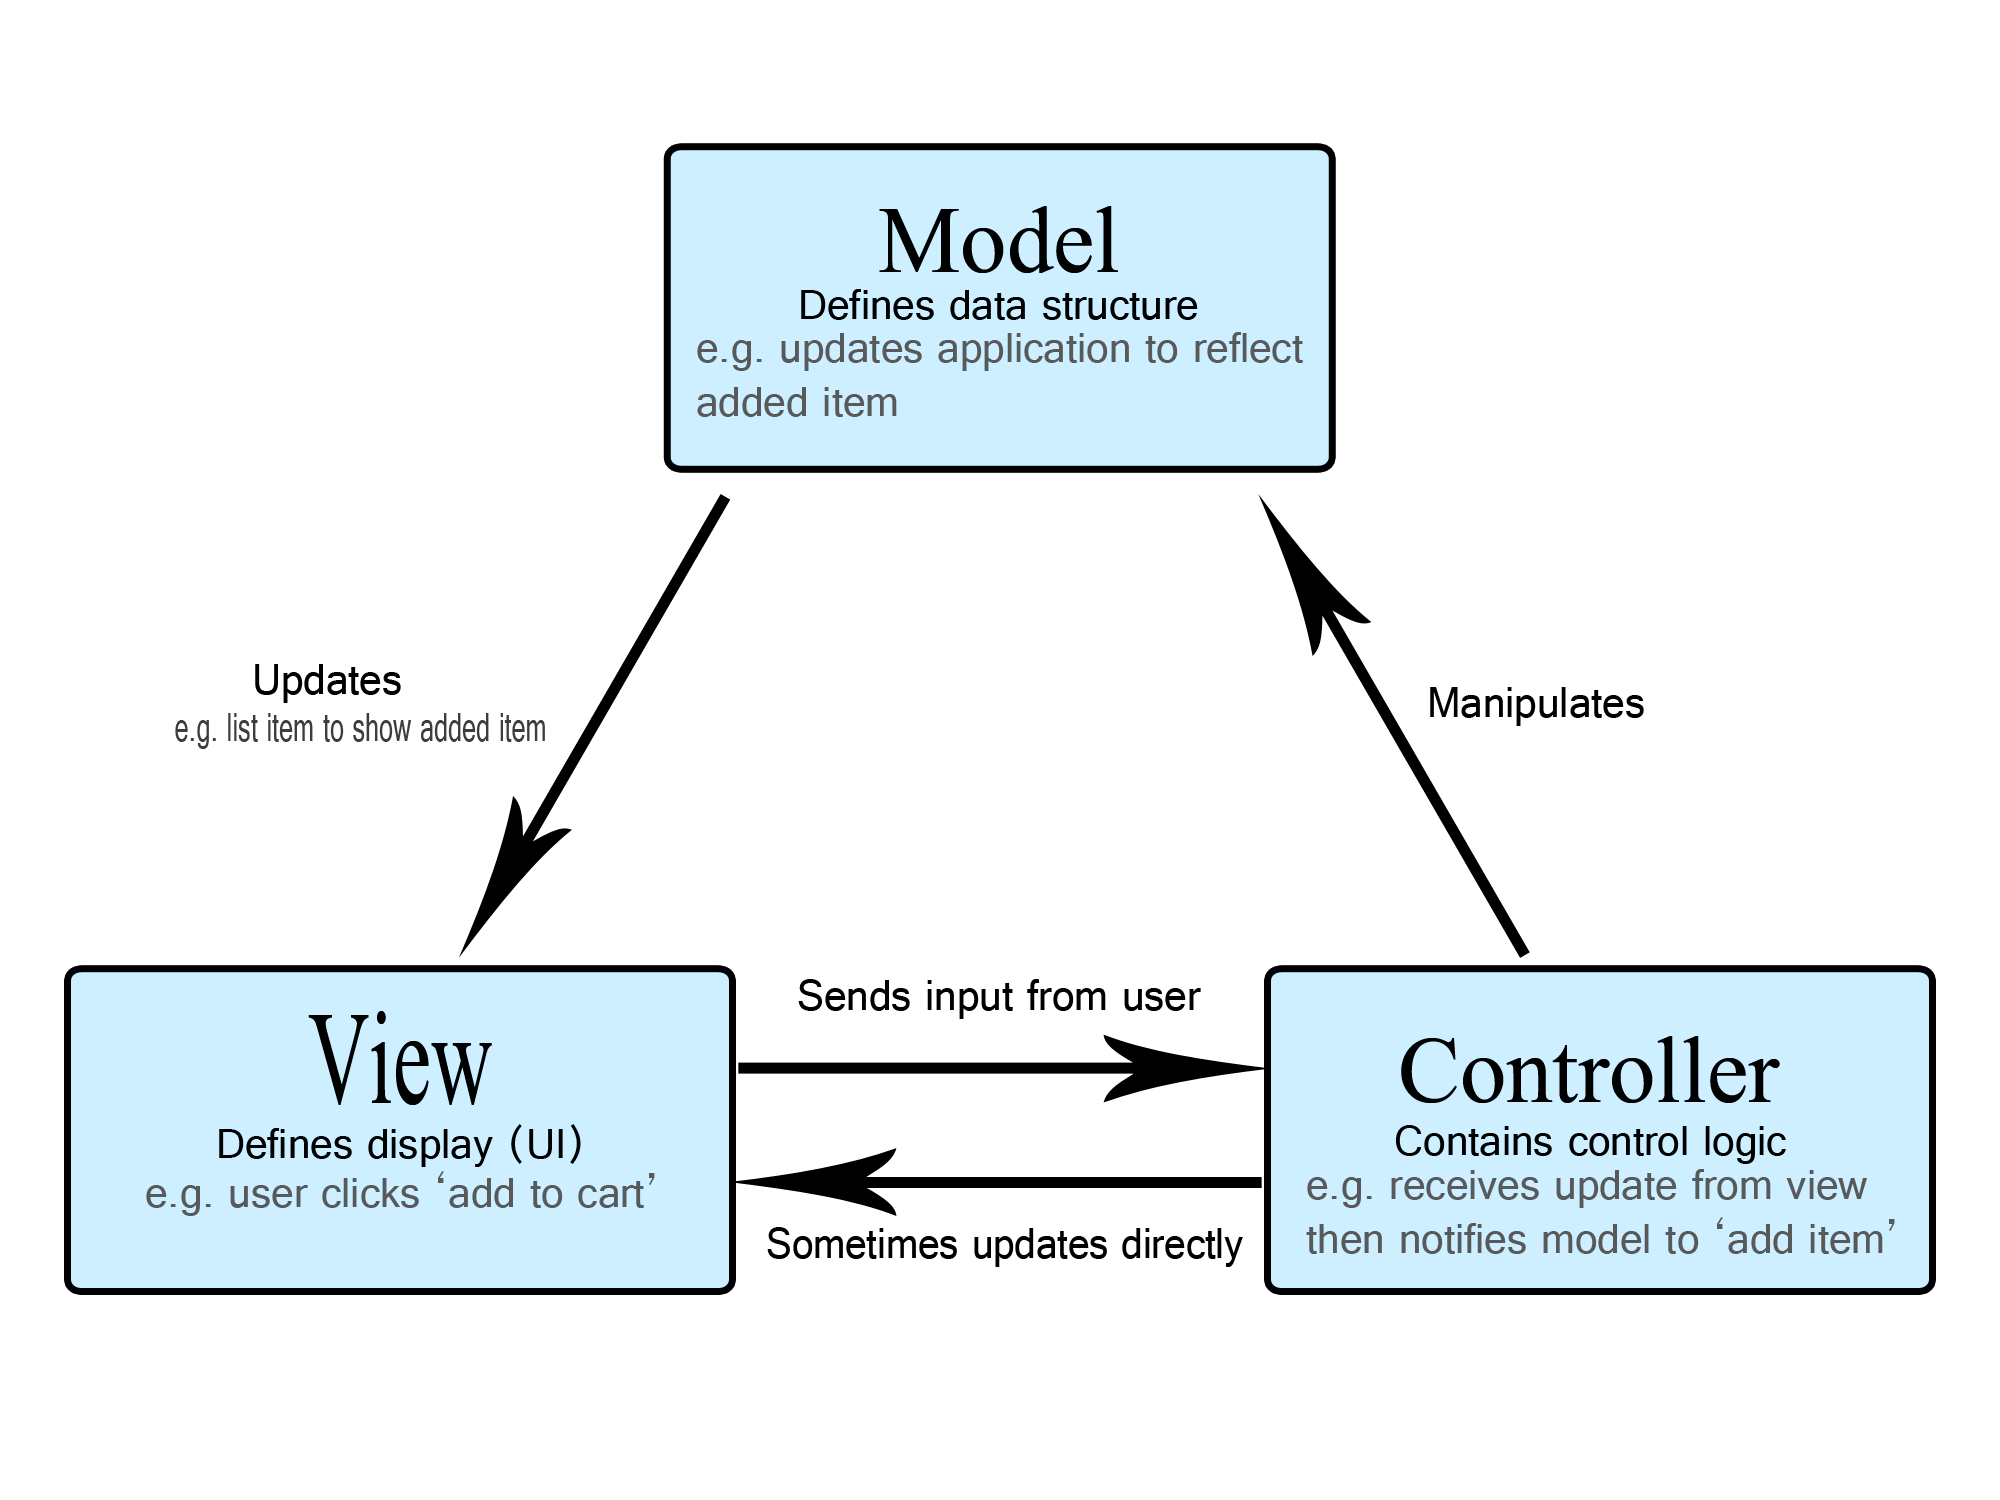
\includegraphics[scale=0.5]{pics/mvc.png}
  \caption{Die Model-View-Controller Pattern \cite{MVCmdn}}
  \label{fig:tech:front:mvc-architecture}
\end{figure}

Welche Daten eine Applikation beinhalten soll, wird über das Model geregelt. Falls sich das Model ändert, werden die Benutzerfläche und manchmal auch der Controller entsprechend geändert. In Angular sind diese Modelle mit den Interfaces (siehe Interfaces \ref{interface})  zu vergleichen.

Die View ist die Benutzeroberfläche des Programms. Der*die Benutzer*in kann mit dieser interagieren und diese verändern. Sie wird aus den Daten des Models erstellt und definiert. In Angular kann diese View mit dem HTML-Template einer Komponente verglichen werden.

In dem Controller werden die Eingaben der Benutzer*innen verarbeitet und die betroffenen Model- und View-Komponenten beeinflusst und verändert. Auch ist es möglich zu bestimmen, welche Views verändert werden sollen und die Daten gegebenenfalls in unterschiedliche Formate anzuzeigen. Die TypeScript-Files in Angular sind vergleichbar mit diesen Controllern.
\cite{MVC}

\subsubsection{Model-View-ViewModel (MVVM)}
Diese Architektur basiert auf dem Konzept des MVC-Patterns. Das MVVM realisiert die “Separation of Concerns” durch die View, ViewModel und Model Komponenten.

\begin{figure} [h t]
  \centering
  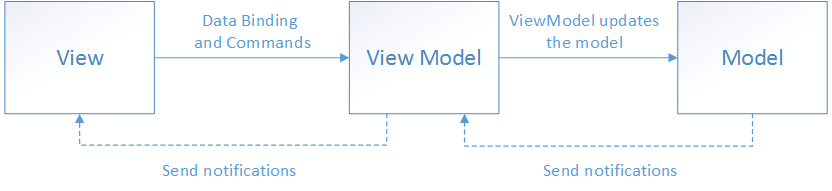
\includegraphics[scale=0.5]{pics/mvvm-pattern.png}
  \caption{Die Model-View-ViewModel Pattern \cite{MVVM}}
  \label{fig:tech:front:mvc-architecture}
\end{figure}

Die View funktioniert hierbei ähnlich wie beim MVC-Pattern, jedoch ist es möglich, dass eine View auch Logik enthält, die Änderungen am Aussehen durchführt. Daher ist das HTML-Template einer Angular-Komponente noch ähnlicher zu dem Konzept einer View aus dem MVVM-Pattern als zu einer View aus dem MVC-Pattern. 

Im ViewModel wird die Funktionalität der Benutzeroberfläche bestimmt. Dabei informiert das ViewModel die View über Änderungen im Model und beliefert es mit Daten. Dieser Vorgang beschreibt das Konzept des Data-Bindings (siehe Data-Binding) in Angular.  

Das Model funktioniert im Grunde gleich wie beim MVC-Pattern, nur wird hierbei nicht die View, sondern das ViewModel über Änderungen informiert. Somit ist das ViewModel das Mittelstück zwischen View und Model.

Angular nutzt hierbei eine Mischung aus beiden Architecture-Patterns. Sie wird durch das Konzept von Komponenten realisiert, auf welches im nächsten Abschnitt näher eingegangen wird. Dabei werden die Parallelen der Patterns erkennbar.
\cite{MVVM}

\subsection{NgModules [M]}\label{sec:NgModules}
\setauthor{Fabian Maar}
NgModules erleichtern die Einbindung von Libraries enorm. Da sich keine externen Files mühsam gedownloadet und eingebunden werden müssen und jeder Import-Prozess fast von selbst geschieht, wird enorm Zeit beim Entwickeln gespart. Außerdem sind alle Importe in chronologischer Reihenfolge gelistet, wodurch ein guter Gesamtüberblick geliefert wird und schnell überflüssige Imports entfernt werden können. Die ständige Erweiterung und die Unterstützung von Third-Party-Libraries, die unter anderem für die 3D-Darstellung verwendet werden, wird ebenfalls von diesen ngModulen ermöglicht. Die Angular-Applikation wird hierbei organisiert und gestartet, in dem die Metadaten wie folgt abgespeichert werden:

\begin{itemize}
  \item Declarations - In dieser Sektion werden alle zugehörigen Komponenten, Direktiven und Pipes deklariert 
  \item Providers - Sie initialisieren wie die Werte bei der Dependency Inection (siehe Dependency Injection \ref{DPI})abgerufen werden \cite{AngularProviders}
  \item Imports - Hier werden alle Libraries und exportierte Modules importiert
  \item Exports - Sie beinhalten alle zu exportierenden Module
  \item Bootstrap - Hierbei wird angegeben welche Komponente beim Anwendungsstart zuerst geladen wird
\end{itemize}

Wie die ngModules verwendet in der 3D-Gallerie-Applikation wurden, wird im Abschnitt Routing oder Landing Page aufsetzen //TODO Referenz nochmals erklärt.
\cite{AngularNgModules}
\cite{AngularNgModulesAPI}
\cite{AngularBuch}


\section{Webstorm [M]}
\setauthor{Fabian Maar}
Webstorm ist eine Entwicklungsumgebung vom Unternehmen JetBrains, die sich auf die Programmiersprache JavaScript spezialisiert hat. Sie wurde besonders für das Arbeiten mit Angular optimiert. Dies zeigt sich durch viele Features, die das Entwickeln von Angular-Projekten erleichtern. So macht es Webstorm möglich, mit nur wenigen Mausklicks eine neue Angular-Dependency oder Komponente zu erstellen. Auch wird die Entwicklungszeit durch intelligente Code-Vervollständigung, Code-Formatierung, einfache Navigation und viele weitere hilfreiche Features deutlich verkürzt.


\section{ThreeJs [L]}
\setauthor{Litzlbauer Lorenz}
\begin{wrapfigure}{r}{0.3\textwidth}
    \begin{center}
      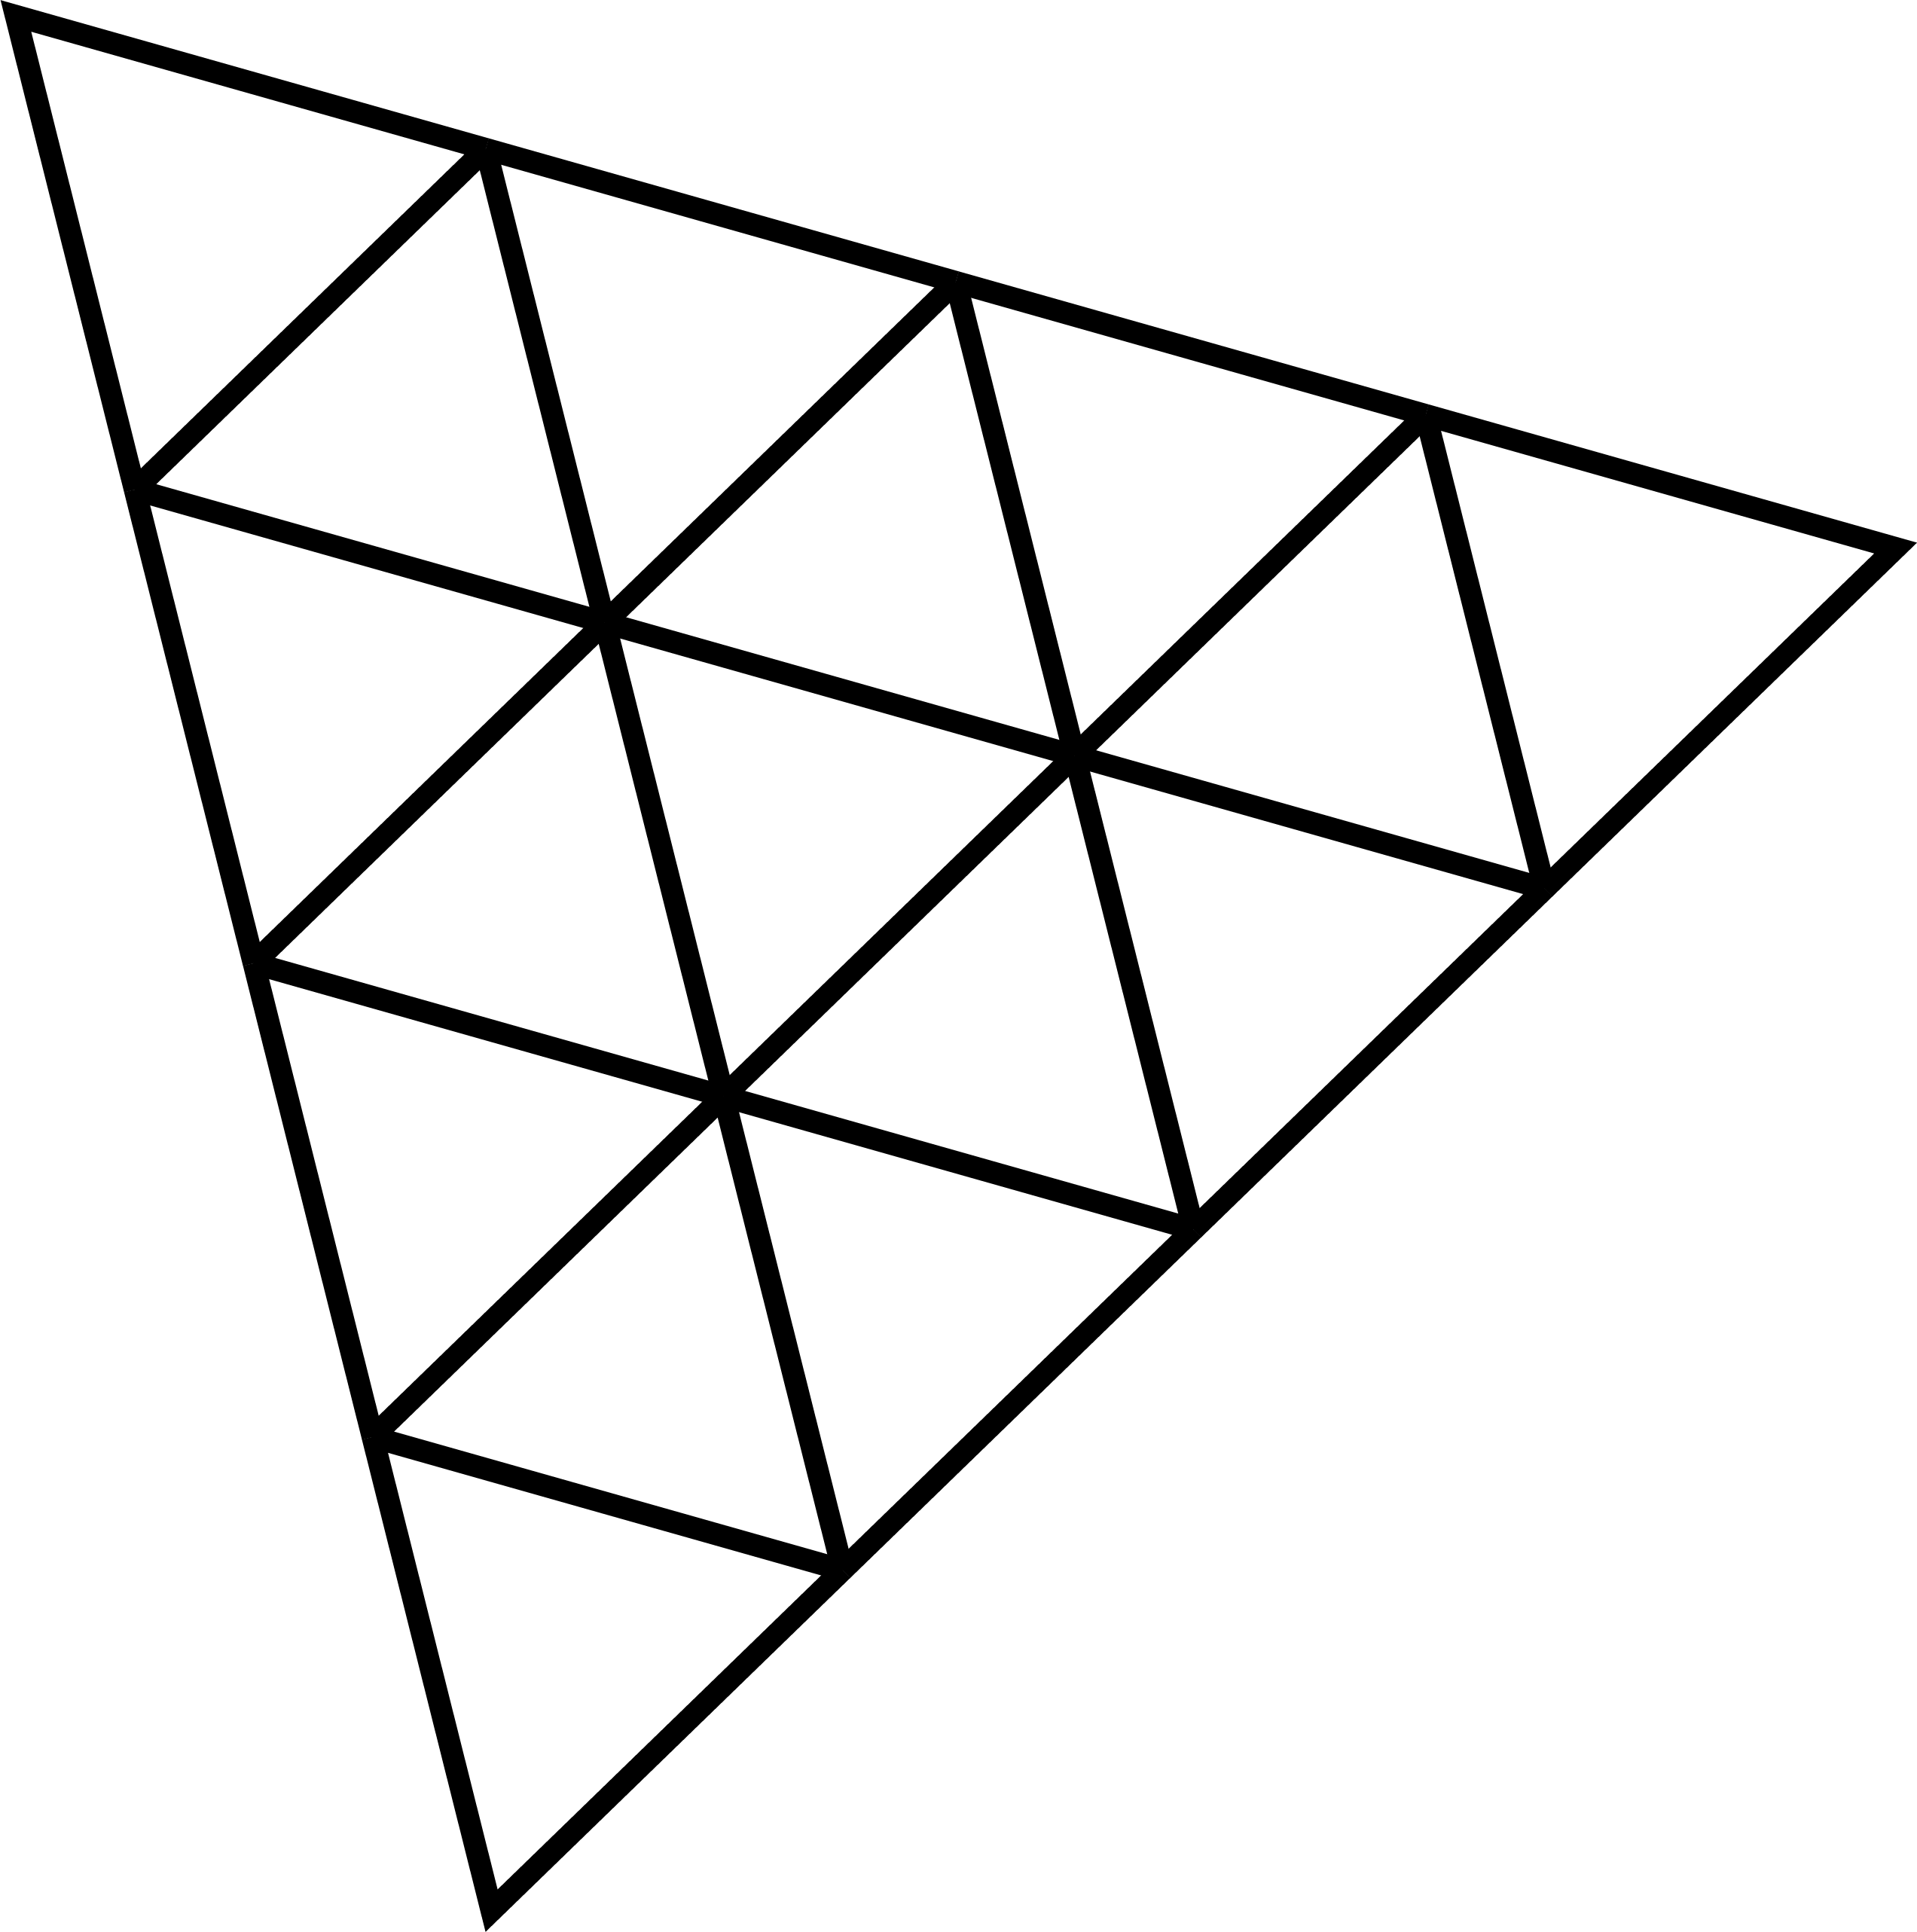
\includegraphics[width=0.2\textwidth]{pics/threeJS.png}
     \caption{ThreeJs Logo}
    \end{center}
\end{wrapfigure}
ThreeJs ist eine JavaScript Library für die Darstellung von 3D-Grafiken im Web. Für die 3D-Darstellung nutzt ThreeJs WebGL (mehr dazu im nächsten Abschnitt \hyperref[ch::ThreeJsDependency]{ThreeJs Dependency}), ein low-level Framework. WebGl hat eine hohe Komplexität. ThreeJs bietet eine Abstraktion zu WebGL, um Anwendungen für 3D-Webanwendungen für Entwickler zugänglicher zu machen. ThreeJs verarbeitet dabei viele Sachen wie die 3D-Szene, Lichter, Schatten, Materialien, Texturen und 3D-Matrix-Rechnungen, die mit WebGl sehr aufwändig wären umzusetzen.

In ThreeJs werden Geometrie, Objekte und Materialien verbunden, um ein 3D-Objekt zu erstellen. Dabei kann die Struktur einer Szene der Abbildung \ref{fig:tech:front:threejsstructure} ähneln. Dort kann beobachtet werden, dass die Scene das Root-Objekt ist. In der Scene werden Objekte wie Meshes, Gruppen, Lichter und 3D-Objekte in einer Baumdatenstruktur gesammelt. Die Daten über die Geometrie, Materialen der 3D-Meshes werden außerhalb der Szene gespeichert und die Meshes referenzieren darauf.

\cite[ThreeJs fundamentals]{ThreeJsFund}

\begin{figure} [h t]
    \centering
    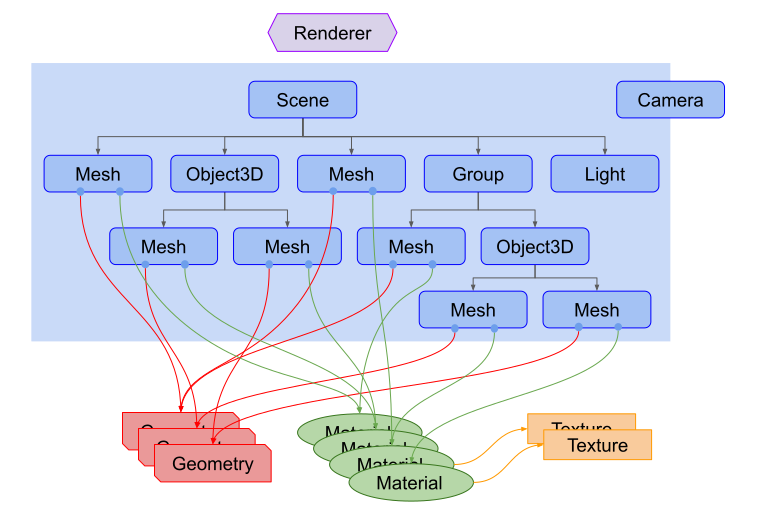
\includegraphics[scale=0.5]{pics/threejs-structure.png}
    \caption{Die Struktur von ThreeJs \cite{ThreeJsFund}}
    \label{fig:tech:front:threejsstructure}
\end{figure}

\subsection{Dependency}
\label{ch::ThreeJsDependency}
Um 3D-Darstellungen zu rendern, benutzt ThreeJs WebGL.

\subsubsection{WebGL}
\label{ch::webgl}
\begin{wrapfigure}{h  r}{0.3\textwidth}
    \begin{center}
      
\includegraphics[width=0.2\textwidth]{pics/WebGL_Logo.png}
     \caption{ThreeJs Logo}
    \end{center}
\end{wrapfigure}
WebGL ist eine lizenzfreie Low-Level-API, die dafür benutzt wird, 3D-Grafiken im Web darzustellen. Sie basiert auf OpenGL ES 2.0 und benutzt auch dieselbe shading language GLSL wie OpenGL. Eine Low-Level-API hat einen höheren Konfigurierungsgrad und lässt sich für spezielle Anwendungsfälle besser anpassen. Der*Die Programmierer*in muss, aber auch ein viel tieferes Verständnis von dem Material haben (im Fall von WebGL Shader-Programmierung, Matrixrechnungen usw.) und hat in der Regel einen viel größeren Programmieranteil als wenn er eine High-Level-API benutzt. Eine High-Level-API  ist besser für allgemeine Anwendungsfälle geeignet.
\cite[WebGl Getting Started]{WebglGettingStarted} \cite{HighlowAPI}


\subsection{Auswahlkriterien}
Es gab verschiedene Auswahlkriterien für die 3D-Web-API, die ausschlaggebend für den Projekterfolg waren:
\begin{compactitem}
  \item Effizienzen der 3D Engine (Hardware Acceleration, RAM-Auslastung)
  \item Benutzerfreundlichkeit (Programmerexperience)
  \item Die Features des Projektes müssen damit umsetzbar sein
  \begin{compactenum}
    \item Das Laden von 3D-Modellen aus 3D-Dateien und aus dem Internet
    \item Video-Texturen support
  \end{compactenum}
\end{compactitem}

\subsubsection{Alternativen 3D Web Apis}
Es gibt viele Technologien, die 3D-Grafiken im Web ermöglichen, wie Three.js, Babylon.js, A-Frame, X3DOM und WebGL

\paragraph{A-Frame}
A-Frame wird von der Mozilla Foundation als OpenSource-Projekt entwickelt. Die 3D-Szene wird durch eine deklarative Sprache mit XML-Syntax definiert. Über die WebVR-API bietet die Libray auch die Möglichkeit, 3D-Szenen durch eine VR-Brille zu erfahren. Bei der 3D-Darstellung setzt A-Frame auf ThreeJs. \cite[A-Frame Wikipedia]{a-frame-wiki}

A-Frame hat ähnliche Funktionen und Leistung im Vergleich zu ThreeJs, da es ja schlussendlich darauf aufbaut. A-Frame sticht bei der VR support hervor (ThreeJs hätte auch eine Unterstützung dafür, diese ist aber schwieriger einzubinden), doch ist das kein unbedingt nötiges Feature. ThreeJs ist ja bereits eine Abstraktion von WebGL. Für das Projekt wird keine weiter Abstraktion gebraucht.

\paragraph{WebGL}
Im Vorherigen Kapitel wurde sich bereits mit WebGL im Kontext mit ThreeJs befasst. In ThreeJs wird WebGL für die 3D-Darstellung gewählt. Doch gibt es auch WebGL als eigenständige Library. \ref{ch::webgl}
Um nur eine einfache 3D-Szene in WebGL darzustellen, muss sehr viel Code geschrieben werden. Denn WebGL übernimmt keine Low-Level-Funktion. Es müssen Matrixrechnungen für die Transformationen von 3D-Objekt Manuel und Vertex buffers, die die Daten der Vertex Positionen, Normaldaten, Farben und Texturen, selbst programmiert werden und das in einer eigenen Programmiersprache. Deshalb war WebGL keine Option für das Projekt.

\subsubsection{Angular Three}
\label{ch:Technologien:AngularThree}
Angular Three ist ein Open Source Projekt von Matt DesLauriers. Es zielt darauf ab die Vorteile von Angular und ThreeJs zu kombinieren. Dabei verbindet es das Prinzip der Komponenten von Angular mit der 3D Darstellung von ThreeJs. 

\begin{lstlisting}[language=html,caption=Angular Three - Komponentenbasiertes 3D Scenen in HTML,label=lst:impl:AngularThreeExampleCode]
<ngt-canvas>
    <ngt-ambient-light intensity="0.5"></ngt-ambient-light>
    <ngt-spot-light [position]="10" angle="0.15" penumbra="1"></ngt-spot-light>
    <ngt-point-light [position]="-10"></ngt-point-light>
  
    <app-cube [position]="[1.2, 0, 0]"></app-cube>
    <app-cube [position]="[-1.2, 0, 0]"></app-cube>
  
    <ngt-soba-orbit-controls></ngt-soba-orbit-controls>
</ngt-canvas>
\end{lstlisting}

\begin{lstlisting}[language=html,caption=Angular Three - App Cube,label=lst:impl:AngularThreeCube]
<ngt-mesh
  (beforeRender)="onCubeBeforeRender($event)"
  (click)="active = !active"
  (pointerover)="hovered = true"
  (pointerout)="hovered = false"
  [scale]="active ? 1.5 : 1"
  [position]="position"
>
  <ngt-box-geometry></ngt-box-geometry>
  <ngt-mesh-standard-material [color]="hovered ? 'turquoise' : 'tomato'"></ngt-mesh-standard-material>
</ngt-mesh>
\end{lstlisting}

Code Beispiele \ref{lst:impl:AngularThreeExampleCode} \ref{lst:impl:AngularThreeCube} \cite{AngularThreeDocumentationFirstScene}

Ein Vorteil von Angular Three ist, dass durch nur wenige Zeilen Code \ref{lst:impl:AngularThreeExampleCode} eine 3D-Szene mit Lichtern und Orientierungsfunktionen erstellt werden kann und die Business-Logik, App-Cube \ref{lst:impl:AngularThreeCube} durch die Verwendung einer Komponente ausgelagert werden kann.

Ein weiterer Vorteil von Angular Three ist die ausführliche Dokumentation mit Codebeispielen. \href{https://angular-three.netlify.app/docs/getting-started/overview}{(link) Angular Three Dokumentation https://angular-three.netlify.app/docs/getting-started/overview}

Wegen der vielen Vorteile hohe Benutzerfreundlichkeit, ähnliche 3D-Leistung zu ThreeJs (Angular Three basiert auf ThreeJs, welches selbst die WebGL-Renderengine benutzt) und wegen der Verbindung von Angular und ThreeJs Features bietet sich die Liberay für das Projekt an.

Mithilfe eines Prototypen ( mehr dazu im Abschnitt \hyperref[ch::ongoing-prototyping]{fortlaufendes Prototyping} ) wurde getestet, ob Angular Three alle Features, die für das Projekt benötigt werden, unterstützen kann, die für das Projekt nötig sind. Dabei wurde festgestellt, dass sich die Library Angular Three für das Projekt nicht eignet. Trotz der vielen Features konnten einige Kriterien nicht erfüllt werden. So wurden beispielsweise 3D-Objekte nicht richtig geladen. ThreeJs Module funktionierten Teilweise nicht, wie die FristPersonControls. 

Weil Angular Three nicht die für das Projekt aufgestellten Anforderungen erfüllt hat, wurde sich dafür entschieden, ThreeJs zu benutzen. ThreeJs hat ähnliche Konzepte und Logik wie Angular Three deswegen fiel dem Team der Umstieg darauf leicht. Diese 3D-Library wurde schlussendlich auch im Projekt verwendet.